\section{Problems}
\label{section:projectSelectionProblems}
\graphicspath{ {./chapter02/FigSolutions} }

\begin{enumerate}
\def\labelenumi{\arabic{enumi}.}
\item
  In your own words, describe the differences between creative, variant,
  and routine designs.
  
 \begin{onlysolution}
 \textbf{[R]}
 \itshape
 Creative designs are typically new and innovative design ideas -- those
that did not exist before. Variant designs are variations of existing
designs, with the intent of improving some aspect of the existing
system. Routine designs are concerned with fairly well-known artifacts
for which there is a well-developed design knowledge base.
  \end{onlysolution}
  
\item
  List three guidelines that should be employed when selecting a
  project.
  
 \begin{onlysolution}
 \textbf{[R]}
 \itshape
 (1) The project must be tied to the mission and vision of the
organization; (2) The project must have payback; (3) The project should
be selected with criterion; (4) The project objectives should be SMART
(Specific, Measurable, Assignable, Realistic, and Time-
Related).
 \end{onlysolution}
  
  
\item
  Assume a customer comes to you with the following
  request---\emph{Design a mechanical arm to pick apples from a tree}.
  What are the assumptions in this statement? Rewrite the request to
  eliminate the assumptions. (This problem was originally posed by
  Edward DeBono {[}Deb70{]}).

  \begin{onlysolution}
  \textbf{[A]}
  \itshape
  This statement contains a solution based on the assumption that a 
  mechanical arm (by means of picking) is the best method for removing 
  apples off of a tree. Therefore, the design space is immediately and 
  needlessly limited. Also, we are unsure if there is a problem with 
  current methods of removing apples. Here is a better statement:
  
  \textbf{“Design a device that can improve the current method of removing apples from a tree.”}
  
  This statement is rightly ambiguous in the sense of not specifying 
  how, or from what, to build this device. This is the type of question 
  and approach that should be sought for establishing a needs statement.
  
   \hspace*{1cm}
  \begin{minipage}{.8\textwidth}
  \textbf{Note:} Including the word “mechanical” 
  \textul{may be} permissible, as it 
  clearly defines a type of device, but does not specify further details 
  or characteristics. This situation poses a fine line between problem 
  and solution.
  \end{minipage}
  \end{onlysolution}

\item
  Assume a customer comes to you with the following
  request---\emph{Design an RS-232 networked personal computer
  measurement system to transmit voltage measurements from a remote
  location to a central server.} What are the assumptions this
  statement? Develop a list of questions that you might ask the customer
  to further clarify the problem statement.

  \begin{onlysolution}
  \textbf{[A]}
  \itshape
  This statement, much like the one confronted in problem 3, is filled 
  with numerous assumptions and solutions. The statement proves troublesome 
  because both the problem (transmit voltages measurements from remote 
  location to central server) and solution (RS- 232 networked personal computer) 
  are given to together. Furthermore, you – as the Engineer – are unsure if 
  the prescribed solutions are the best decisions for this particular problem. 
  In order to dissect the statement and get to the actual problem, a list of 
  questions must be asked.
  
  \underline{\textit{\textbf{Sample Questions}}}
  \begin{itemize}
    \item What is the purpose of this transmission system?
    \item Why are voltage measurements currently being sent? What do they represent?
    \item How are the measurements currently being made?
    \item What are the problems with the current system?
    \item What do you like about the current system?
    \item What type of atmosphere will this device most likely be engaged in?
    \item Do you plan to implement multiple measurement systems?
    \item Why use RS-232?
    \item What is the purpose of the central server?
    \item What are the voltage measurements of?
  \end{itemize}
  
     \hspace*{1cm}
  \begin{minipage}{.8\textwidth}
  \textbf{Note:} The questions given here are variations on those presented in 
  the book to ask the client when starting into a new project. The objective 
  in asking this question is to get practice in asking these questions. Students 
  are often hesitant to ask questions, particularly if they are working with an 
  industrial sponsor. It help to give them practice in do this before they meet 
  with their customer.
  \end{minipage}
  \end{onlysolution}

\item
  Describe what is meant by a marketing requirement.

  \begin{onlysolution}
  \textbf{[R]}
  \itshape
  A marketing requirement is a statement that describes a need in the language 
  of the end-user or customer. It should describe what the system should do, not 
  necessarily how it will be accomplished.
  \end{onlysolution}

\item
  What is the purpose of an objective tree and how is it developed?
  
  \begin{onlysolution}
  \textbf{[R/A]}
  \itshape
  The objective tree is a graphical representation of the customer/end-user needs 
  in a hierarchical layout. It is developed by determining the customer needs 
  (through interviews, observations, etc.) and then translating the results of 
  that into a set of specified needs. The needs are categorized into a hierarchy 
  which is represented in the objective tree. The categorization is based upon 
  functionality, not importance.
  \end{onlysolution}

\item
  The needs for a garage door opener have been determined to be: safety,
  speed, security, reliability, and noise. Create a pairwise comparison
  to determine the relative weights of the needs. Apply your judgment in
  making the relative comparisons.

  
  \begin{onlysolution}
  \textbf{[A]}
  \itshape

\begin{tabular}{ll}
\textbf{DEVICE:} 	& Garage Door Opener \\ 
\textbf{NEEDS:}	& Safety, Speed, Security, Reliability, and Noise \\ 
\end{tabular}

	\begin{tabular}{l|l|l|l|l|l|l} \\
		& Safety	& Speed	& Security	& Reliability	& Noise		& Total \\ \hline
Safety	&	X		&	1		&	1		&	0.5		&		1	&	3.5		\\ \hline
Speed	&	0		&	X		&	1		&	0		&	0.5		&	1.5		\\ \hline
Security	&	0		&	0		&	X		&	0.5		&	1		&	1.5		\\ \hline
Reliability&	0.5		&	1		&	0.5		&	X		&	1		&	3		\\ \hline
Noise	&	0		&	0.5		&	0		&	0		&	X		&	0.5		\\ 
	\end{tabular}
  
	\begin{tabular}{l l} \\
	Most Important 	& Safety		\\ 
					& Reliability		\\ 
					& Security		\\ 
					& Speed		\\ 
	Least Important & Noise			\\
	\end{tabular}					
	
     \hspace*{1cm}
  \begin{minipage}{.8\textwidth}
  \textbf{Note:} There is no single solution, and the results are somewhat 
  subjective. However, safety should always be of the highest concern in 
  such an application. The objective of this problem is to demonstrate 
  that students can create a matrix, make it consistent, and compute the 
  scores.
  \end{minipage}
  \end{onlysolution}

\item
  Consider the design of an everyday consumer device such as computer
  printer, digital camera, electric screwdriver, or electric toothbrush.
  Determine the customer needs for the device selected. The deliverables
  should be: 1) marketing requirements, 2) an objective tree, and 3) a
  ranking of the customer needs using pairwise comparison.
  
  \begin{onlysolution}
  \textbf{[A]}
  \itshape
  \emph{Note:} The objective of this question is to give the individual 
  (or preferable a small-team) practice in identifying the needs. Fairly 
  simple and common products should be used as a first step. This can be 
  a very good exercise for the class. Each team could select its own product 
  and then some teams can present the results to the class. Or several or 
  all teams could work on the same project, with a reporting session, where 
  a team presents their findings and the others critique them.
  
  \underline{Consumer Device Selected:} \textbf{Cellular Phone}
  
  \textbf{Need:} With today’s high-paced world, immediate contacts are essential. Therefore,
  excellent cell phone design, implementation, and construction are a must.
  \begin{enumerate}
  \def\labelenumi{\arabic{enumi}.}
    \item \underline{\textbf{Marketing Requirements}}
• The system will be lightweight.\\
• The system will withstand abusive treatment (dropping, running over, etc.).\\
• The system will be comfortable and ergonomic.\\
• The system will have high-quality audio encoding and decoding.\\
• The system will not have to be frequently charged.\\
• The system will have good signal pickup.\\
• The system will survive from weathering (sun, rain, etc.).\\
• The system will be easy-to-use.\\
• The system will be able to connect to and browse the internet.\\
• The system will contain as few buttons as possible.

    \item \underline{\textbf{Objective Tree}}

	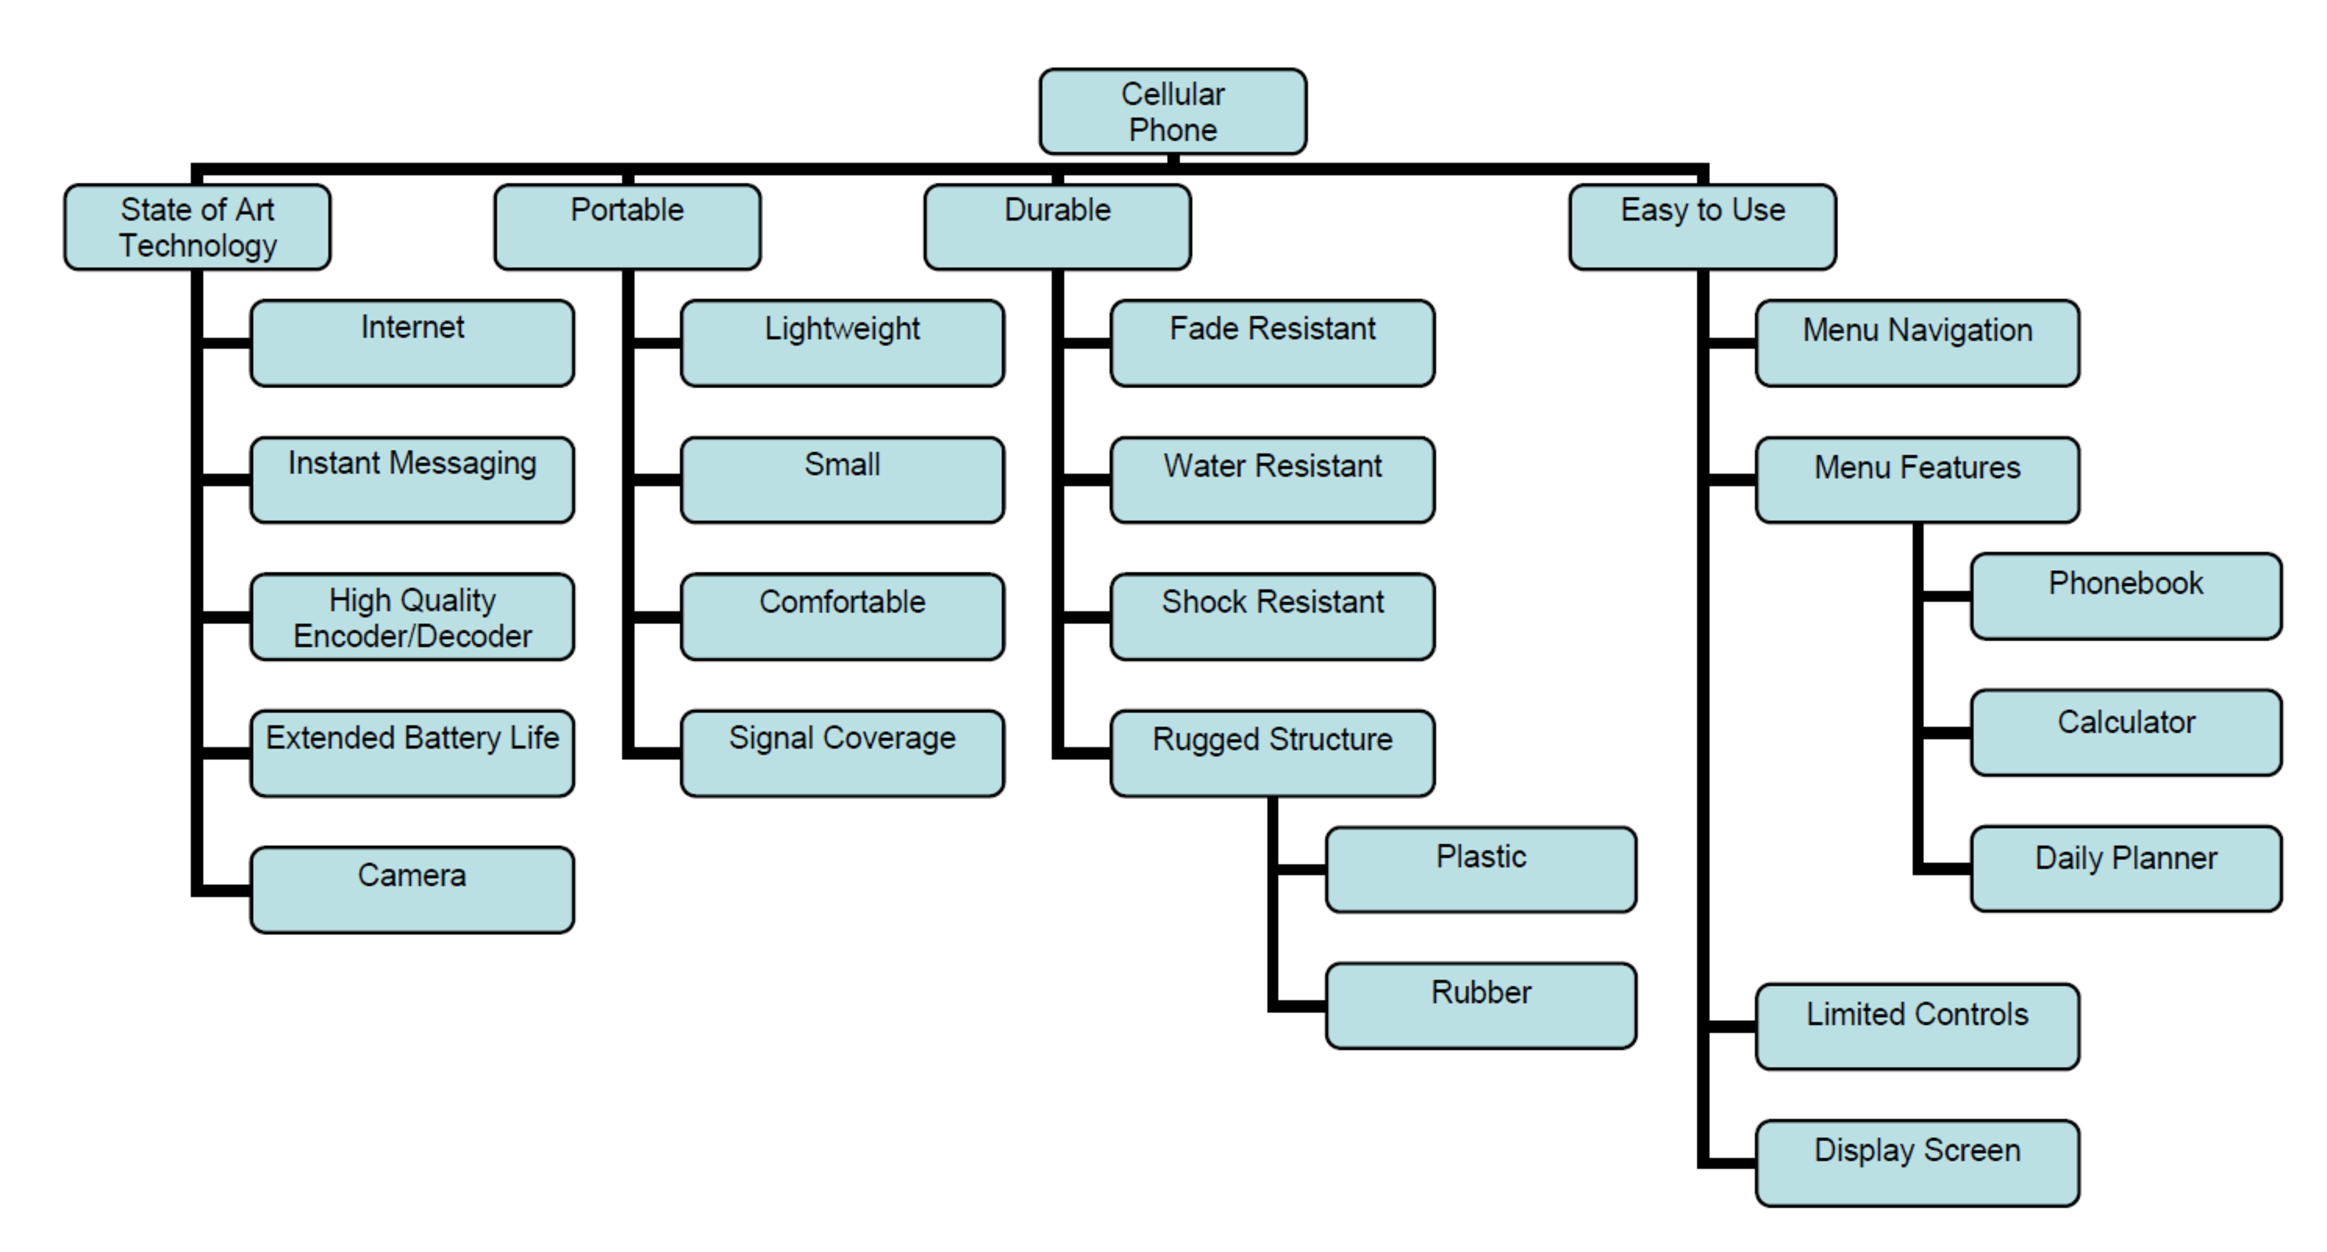
\includegraphics[width=\textwidth]{phoneObjectiveTree}

 
   \item \underline{\textbf{Ranking of Customer Needs}}   
    \begin{table}
    \caption{Cell Phone Attributes}
    \begin{tabular}{c|c|c|c|c|c}
    				& Technology	& Portable	& Durable	& Easy-to-Use 	& Total			\\ \hline    			
	Technology	& X 			& 0.5		& 0.5		& 0.5			& 1.5 			\\ \hline    			
	Portable		& 0.5 			& X			& 0.5		& 0.5			& 1.5	 			\\ \hline    			
	Durable		&  0.5			& 0.5		& X			& 0				& 1 			\\ \hline    			    
	Easy-to-use	&  0.5			& 	0.5		& 1			& 	X			& 2 			\\ \hline    			
	\end{tabular}
	\end{table}


    \begin{table}
    \caption{State of the art technology}
    \begin{tabular}{c|c|c|c|c|c|c}
    				& Internet		& Text		& Audio	& Battery	 	& Camera	& Total			\\ \hline    			
	Internet		& X 			& 0.5		& 0			& 0				& 1			& 1.5 			\\ \hline    			
	Text			& 0.5 			& X			& 0			& 0				& 0	 		& 0.5		\\ \hline    			
	Audio		&  1			& 1			& X			& 0.5			& 1 		& 3.5		\\ \hline    			    
	Battery		&  1			& 1			& 0.5		& 	X			& 1 		& 3.5		\\ \hline    			
	Camera		& 0				& 1			& 0			& 0				& X 		& 1	
	\end{tabular}
	\end{table}
			
    \begin{table}
    \caption{Portable}
    \begin{tabular}{c|c|c|c|c|c}
    				& Lightweight	& Coverage	& Small		& Comfortable 	& Total			\\ \hline    			
	Lightweight	& X 			& 0			& 0.5		& 0.5			& 1 			\\ \hline    			
	Coverage	& 1	 			& X			& 1			& 1				& 3	 			\\ \hline    			
	Small		&  0.5			& 0			& X			& 0				& 0.5 			\\ \hline    			    
	Comfortable	&  0.5			& 0			& 1			& 	X			& 1.5 			\\ 			
	\end{tabular}
	\end{table}

    \begin{table}
    \caption{Durable}
    \begin{tabular}{c|c|c|c|c|c}
    				& Fade Res.	& Water Res.	& Shock Res.	& Rugged 	& Total			\\ \hline    			
	Fade Res.	& X 			& 0			& 0				& 0.5			& 0.5 			\\ \hline    			
	Water Res.	& 1	 			& X			& 0.5			& 1				& 2.5			\\ \hline    			
	Shock Res.	&  1			& 0.5		& X				& 0.5			& 2 			\\ \hline    			    
	Rugged		&  0.5			& 0			& 0.5			& 	X			& 1 			\\ 			
	\end{tabular}
	\end{table}



    \begin{table}
    \caption{Easy To Use}
    \begin{tabular}{c|c|c|c|c|c}
    				& Navigation	& Features	& Lim. Ctrls.	& Display 	& Total			\\ \hline    			
	Navigation	& X 			& 0.5		& 0.5			& 0			& 1 			\\ \hline    			
	Features	& 0.5	 		& X			& 0.5			& 0			& 1			\\ \hline    			
	Lim. Ctrl.	&  0.5			& 0.5		& X				& 0			& 1 			\\ \hline    			    
	Display		&  1			& 1			& 1				& 	X		& 3 			\\   			
	\end{tabular}
	\end{table}

    \begin{table}
    \caption{Menu Features}
    \begin{tabular}{c|c|c|c|c}
    				& Phonebook	& Calculator& Planner	 	& Total			\\ \hline    			
	Phonebook	& X 			& 1			& 1				& 2 			\\ \hline    			
	Calculator	& 0	 			& X			& 0				& 0			\\ \hline    			
	Planner		&  0			& 1			& 1				& 1 			\\   			
	\end{tabular}
	\end{table}


    \begin{table}
    \caption{Rugged Structure}
    \begin{tabular}{c|c|c|c}
    				& Plastic	& Rubber	& Total			\\ \hline    			
	Plastic	& X 			& 0.5		& 0.5 			\\ \hline    			
	Rubber	& 0.5	 		& X			& 0.5			\\ \hline    			
	
	\end{tabular}
	\end{table}
	
   \item \underline{\textbf{Ranking}}  
   
\begin{tabular}{ll}
Most Important 	& Extended Battery Life and Audio Encoding/Decoding (3.5)			\\ 	
 & Signal Coverage and Display Screen (3)			\\    	
 &Water Resistant (2.5)			\\ 	
 & Easy to Use, Shock Resistant, and Phone Book Feature (2)			\\ 	
 & State of the Art Technology, Internet, Portable, and Comfortable (1.5)			\\  	
 &Durable, Camera, Lightweight, Rugged, Menu Navigation, Menu Features, Limited Controls, and Daily Planner (1)			\\ 	
& Instant Messaging, Small, Fade Resistant, Plastic, and Rubber (0.5)			\\ 	
Least Important & Calculator (0)			\\ 	
\end{tabular}


  \end{enumerate}
  \end{onlysolution}

\item
  \textbf{Project Application.} Select criteria to be applied for
  selecting a project concept as shown in Example~\ref{example:projectSelectionModel}
  then brainstorm and search to generate project concepts. Rank the top three to five
  concepts against the criteria as presented in Example~\ref{example:projectSelectionModel}.

  \begin{onlysolution}
  \textbf{[P]}
  \itshape
  \emph{Note:} If the teams are being allowed to select the project, this is a good exercise 
  to get them to focus on criteria for project selection. Conflict often develops between 
  team members over which project to pursue, and this provides an opportunity to examine the 
  merits of different projects. Criteria to consider are: cost, time to completion, team member 
  skills, probability of success, interest in the project, etc.
  \end{onlysolution}

\item
  \textbf{Project Application.} Determine the needs for the project
  selected. The result should be list of marketing requirements, an
  objective tree, and a ranking of the needs.

  \begin{onlysolution}
  \textbf{[P]}
  \itshape
  \emph{Note:} The objective here is the same as question 8, with difference being that it 
  is applied to the capstone design project. A difficulty here could be that the customer may 
  not be as easily identifiable, an example being a design competition. If the team is developing 
  a new and creative product idea, they should be able to do this. If they are working on an 
  industry sponsored project, they should also be able to do this. In the case of design competition
  or another type does not lend itself as well, the team still should be able to develop an adequate 
  objective tree based on the project rules and their knowledge of the subject. We have had teams be 
  very creative in finding ways to identify the customer needs from conducting web-based surveys on 
  bulletin boards and to conduct focus groups with other students on campus.
  \end{onlysolution}

\item
  \textbf{Project Application.} Conduct a research survey for your
  project using the guidance presented in Section~\ref{section:needs-identification}. The result should
  be a report summarizing the results of the survey.

  \begin{onlysolution}
  \textbf{[R]}
  \itshape
    No Answer Provided.
  \end{onlysolution}

\item
  \textbf{Project Application.} Develop a Problem Statement for your
  project concept as outlined in Section~\ref{section:project-application-the-problem-statement}. 
  Apply the processes presented in the chapter as appropriate.

  \begin{onlysolution}
  \textbf{[P]}
  \itshape
  \textbf{Note:} We typically have the teams complete the simple \textul{Problem Statement} similar to those 
  in Examples 2.1-2.3 in the text. Along with this they submit a justification for the team they 
  have selected (\textul{Team Proposal}) that identifies who the members are and what objectives/skills they 
  bring to the team.
  Once the basic Problem Statement and Team Proposal are completed and reviewed by the instructor, 
  it is then followed by a more detailed submission of the \textul{Extended Problem Statement} that is presented 
  in the Project Application Section. This integrates all of the material from Chapter 2. In term of 
  research, the goal here is to provoke the team to conduct research up-front and show they understand 
  what is going on. In our experience, this is often overlooked, and teams regret it later. In our course, 
  we typically get a 3-6 page report summarizing their findings. Our goal is to determine their level of 
  understanding based upon that. All of this makes up part of the final design report submitted at the end 
  of the project.


\textbf{Additional In-Class Exercise}
\noindent\rule[0.5ex]{\linewidth}{1pt}

The following exercise is one we use early on in the class to generate
project ideas. The class is usually capable of generating at least one
idea per minute, and we often get 40-50 ideas in a session.

As a class, the objectives are as follows:

\begin{quote}
•Generate a minimum of 40 project ideas.\\
•Every single student in the class must offer at least on idea.\\
•If the two above criteria are met, then everyone in class gets a 10
point (100\%) quiz grade. Otherwise, no grade recorded.
\end{quote}

\textul{Rules of Brainstorming}

\begin{quote}
1.No criticism or judgment of idea\\
2.Wild ideas are encouraged.\\
3.Quantity is stressed over quality.\\
4.Build upon and modify the ideas of others.\\
5.All ideas are recorded.
\end{quote}

\textbf{Note:} Another option is to present a particular problem
or application area and have the teams students generate ideas based
upon them.

\textbf{CENBD/EE BD 480 - Engineering Design Concepts}\\
\textbf{\textul{Penn State Erie, The Behrend College}}

\begin{center}
\textbf{Background and Technology Survey Instructions}
\end{center}

You should consult with your supervising faculty member when developing
this section of the report. Each project is unique.

The objectives of this section are to:
\begin{quote}
•Provide your audience (faculty, project sponsors, other students, etc)
with sufficient background so that they understand the problem the team
plans to solve.\\
•Demonstrate that the team has a sufficient understanding of the problem
to proceed to the next stage of development.\\
•Demonstrate that the team has conducted research and understands the
technology relevant to this project -- namely, related solutions to the
problem and their limitations.\\
•Depending on the project, you should also conduct searches on the US
patent database for similar technologies.\\
•To describe what is new/unique in the proposed design.\\
•To provide additional supporting information that for the Need and
Objective statements.
\end{quote}

Pointers:
\begin{quote}
•If it is an industry sponsored project, you will need to provide a
clear overview of the problem and any related processes. You should also
indicate why it is important to the organization -- what benefit it will
provide.\\
•You may provide more detail on the need for the project. For example,
if this has market potential, indicate what the size of the market is.
If you are preventing injuries -- how many injuries are there per year?
Supporting statistics are always great to demonstrate the need.\\
•If there are similar systems out there, describe limitations of current
designs or technology. Benchmarking or strength/weaknesses analyses of existing
technologies are powerful.\\
•Describe any basic theory to be described regarding the technology. For
example, say you are designing a flywheel energy storage system -- you
should describe the basics of how flywheel energy systems work -- what
are the major systems, etc.\\
•Pictures always help - be sure to provide a description of diagrams.
\end{quote}

On the writing itself:
\begin{quote}
•This is expected to be well-written prose.\\
•You \textbf{must} provide a reference section. Reference all sources
used -- do not plagiarize. If you use a figure that is not yours, you
must provide a clear reference as to where it came from -- if not it is
plagiarism (in which case you get a zero and reported for academic
integrity hearings).\\
•Follow the same format for references as used in the class textbook.
Make sure that you reference web pages properly.\\
•All figures and tables must be labeled. Follow the same format used in
the book for labeling and referring to figures and tables.\\
•This should be concise 3-4 pages in length. You cannot exceed 4 pages
of 11 point with 1'' margins.\\
\end{quote}

\begin{center}
\textbf{Format for the report}
\end{center}

Use 12 point Times New Roman bold for the headings of the section. 11 pt
for text, 1.5 spacing between paragraphs.

\textbf{Title}

\textbf{Team Members}

\textbf{1. Need}\\
Text goes here -- it should be 11 pt, Times- New Roman single spaced.
Use 1.5 spacing between the paragraphs.

\textbf{2. Objective}\\
Text goes here -- it should be 11 pt, Times- New Roman single spaced.
Use 1.5 spacing between the paragraphs.

\textbf{3. Background and Technology Survey}\\
Text goes here -- it should be 11 pt, Times- New Roman single spaced.
Use 1.5 spacing between the paragraphs.

\textbf{4. Marketing Requirements and Objective Tree}\\
List the marketing requirements (numbered), Objective tree, and a
summary of the ranked needs.

\textbf{References}

\textbf{Appendix -- Ranking of Needs}\\
List the marketing requirements (numbered), Objective tree, and a
summary of the ranked needs.
  \end{onlysolution}
\end{enumerate}
